\documentclass[11pt]{article}
\usepackage[review]{acl}
\usepackage{times}
\usepackage{latexsym}
\usepackage[T1]{fontenc}
\usepackage[utf8]{inputenc}
\usepackage{microtype}
\usepackage{inconsolata}
\usepackage{graphicx}
\usepackage{booktabs}
\usepackage{amsmath,amssymb,amsthm}
\usepackage{xcolor}
\newtheorem{proposition}{Proposition}
\newcommand{\pL}{\texttt{\textbackslash p\{L\}}}
\newcommand{\pM}{\texttt{\textbackslash p\{M\}}}
\newcommand{\RO}{\textsc{R0}}
\newcommand{\RI}{\textsc{R1}}
\newcommand{\RII}{\textsc{R2}}
% Anonymous review version of main.tex: identical except the acl option, the author block and this macro.
\newcommand{\artifactnote}{Code, results, analysis plan and tokenizers: anonymised for review.}

\title{Merge-Based Vocabulary Extension Stalls at the Pre-Tokenizer:\\ Repairing Deployed LLMs for Nepali, and What It Costs}

\author{Anonymous submission}

\begin{document}
\maketitle

\begin{abstract}
Many widely used open LLMs split text with a regular expression that treats a word as a run of Unicode letters. Devanagari vowel signs are combining marks, not letters, so this letters-only regex cuts every Nepali word apart before tokenization, and Nepali costs current open models that use it $2.6$--$5.8\times$ as many tokens as English. Vocabulary extension, the standard way to adapt a deployed model to a new language, cannot cross these cuts: for Llama-3 and Qwen3 no number of appended merges takes the Nepali premium below about $2.2\times$, and ten released extensions of Llama-3 and Qwen models for six Indic and Southeast Asian scripts already sit within 4\% of their floors. We give a two-substitution repair of the deployed regex that provably leaves the token ids of every input with no combining mark and no Devanagari code point unchanged, which includes all ASCII English and code. Combined with continued-BPE extension, it brings Nepali to $1.01\times$ English at 32{,}000 new merges and $0.95\times$ at 64{,}000, and gives the same pattern for seven other languages, with no change for two languages whose scripts have no combining marks. In controlled continued pretraining of Llama-3.2-1B and Qwen3-0.6B on 2\,GB of text, keeping the original vocabulary gives the best held-out Nepali bits per byte at this budget. Against standard extension, the repaired tokenizer is 2--6\% worse on Nepali but needs 26\% less training compute, is slightly better on English, and generates Nepali about 1.5$\times$ faster; training the new embeddings first narrows its gap. We also document an evaluation artifact: scoring after a beginning-of-sequence token that continued pretraining never used changes the comparison between arms. We release the tokenizers, a diagnostic tool, code and pre-registration.
\end{abstract}

\section{Introduction}

A Nepali sentence costs a deployed open LLM several times more tokens than its English translation: $4.42\times$ under the Qwen3 tokenizer and $4.76\times$ under the \texttt{cl100k} tokenizer shared by Phi-4, OLMo-2 and Granite-4.1, measured on parallel FLORES-200 text (\S\ref{sec:audit}). Every extra token is paid for in money, latency and context length, so the premium is a recurring cost for the tens of millions of people who speak Nepali.

A large share of this premium has a known, mechanical cause. GPT-2-style pre-tokenizers split text with a regular expression whose word class is \pL{}, one or more Unicode \emph{letters}~\citep{gpt2encoder}. We call this the \emph{letters-only regex}. Devanagari writes its dependent vowel signs, virama, anusvara and candrabindu as combining \emph{marks} (\pM{}), so the regex starts a new pre-token at every vowel sign, and byte-pair encoding can never merge across that boundary. \citet{regmi2026vowel} formalised this as a training-free lower bound on fertility. They showed that widening the word class to \texttt{[\textbackslash p\{L\}\textbackslash p\{M\}]+} cuts Nepali from 4.78 to 1.58 tokens per word, and found the letters-only class in 63\% of the 1{,}345 Hugging Face text-generation repositories they classified. OpenAI's \texttt{o200k} tokenizer and Meta's Llama-4 already ship a mark-aware class.

That result concerns tokenizers trained from scratch. Practitioners rarely train from scratch: the standard way to adapt a deployed model to a new language is \emph{vocabulary extension}, which adds target-language tokens, initialises their embeddings and continues pretraining~\citep{tejaswi-etal-2024-exploring,yamaguchi2026lowres,purason-etal-2026-teaching,smith2026inplace}. This paper asks what happens when that recipe meets the pre-tokenizer.

\paragraph{Vocabulary extension cannot cross a pre-tokenizer boundary.} New merges, like old ones, act only within pre-tokens. A model whose regex shatters Nepali into $P$ pre-tokens can never encode it in fewer than $P$ tokens, however many merges are appended. Released extensions already sit on this bound: ten published extensions of Llama-3 and Qwen models for six scripts written with combining marks use only 1.3--3.6\% more tokens than their pre-token count (Figure~\ref{fig:released}). The resulting lower bound on the Nepali/English premium, the \emph{pre-token floor} (defined in \S\ref{sec:audit}), is $2.19\times$ for Llama-3 and $2.17\times$ for Qwen3 (\S\ref{sec:ceiling}). Llama-3 already sits at $2.58\times$, so the standard recipe can remove at most 15\% of its current premium. The floor is also above the premium of \texttt{o200k} ($1.61\times$): no amount of vocabulary extension can bring a letters-only model to parity with GPT-4o's tokenizer on Nepali. The three published extension studies of these model families for Indic and other abugida languages that we inspected kept the letters-only regex~\citep{yamaguchi2026lowres,purason-etal-2026-teaching,smith2026inplace}. One of them expands LFM2, whose released 64k tokenizer costs $5.77\times$ on Nepali (\S\ref{sec:audit}); any such expansion of it keeps a floor of $2.15\times$.

\paragraph{An English-lossless repair.} The fix is to change the regex of the deployed model. Changing a pretrained model's pre-tokenizer usually changes how it tokenizes everything, including English~\citep{dagan2024getting}. We use a minimal edit, the \emph{repaired regex}, that does not. For any input with no combining mark and no code point in U+0900--U+097F, which includes all ASCII text, the repaired tokenizer produces exactly the original token ids (Proposition~\ref{prop:lossless}). We then learn new merges by continued BPE~\citep{purason-etal-2026-teaching} restricted to Devanagari outputs. The repaired tokenizers give identical token ids on all 1{,}012 FLORES devtest sentences in English, Russian and Amharic. Before any training, the resized model's logits over the original vocabulary are identical to the base model's up to float error ($<10^{-4}$) on an English probe sentence.

\paragraph{Contributions.}
\begin{enumerate}
  \setlength\itemsep{0pt}
  \item An audit of 33 released tokenizers (24 distinct), with each premium decomposed into a regex factor and a vocabulary factor, and the pre-token floor of every letters-only tokenizer (\S\ref{sec:audit}).
  \item Evidence that the floor binds vocabulary extension in practice: a released Telugu extension of Llama-3 sits within 2\% of its floor, and continued BPE under the letters-only regex stalls at the floor for both of our models (\S\ref{sec:ceiling}, \S\ref{sec:compression}).
  \item A minimal, provably English-lossless repair of a deployed model's pre-tokenizer, with continued-BPE extension and an exactness check on the resized model (\S\ref{sec:method}).
  \item A controlled comparison of \RO{} (no extension), \RI{} (extend) and \RII{} (repair + extend) on Llama-3.2-1B and Qwen3-0.6B-Base under identical data, merge budget and optimisation, scored per byte (\S\ref{sec:results}).
  \item Released tokenizers, code and pre-registration.\footnote{Pre-registration commits are timestamped before any continued-pretraining result was observed; see Appendix~\ref{app:prereg}.}
\end{enumerate}

\section{Related work}
\label{sec:related}

\paragraph{Tokenization premiums.} Tokenizers trained mostly on English encode other languages in more tokens, and since commercial models bill per token, those languages pay more for the same content~\citep{petrov2023unfairness,ahia-etal-2023-languages}. Recent work documents such premiums for African, European, Indic and other languages~\citep{lundin-etal-2026-token,ovcharov2026european,somide2026african,tamang2024evaluating}, including a Nepali/English ratio of $4.79\times$ for \texttt{cl100k} on 150 parallel passages~\citep{kadariya2026nepali}. \citet{srivastava2026tokenizertax} and \citet{mandarapu2026ledger} measure large Indic premiums on FLORES-200, and the former reports that \texttt{o200k} cuts the mean Indic premium from $8.0\times$ to $2.1\times$; neither attributes the change to the regex. We report the premium as a sentence-level token ratio on parallel FLORES-200 text~\citep{goyal-etal-2022-flores,nllb2022}, following \citet{petrov2023unfairness}, and add paired bootstrap intervals. Fewer tokens do not by themselves make a better model~\citep{schmidt-etal-2024-tokenization}, which is why we test the repair with continued pretraining.

\paragraph{Pre-tokenization of combining marks.} That GPT-2-style regexes split Indic words at vowel signs was reported publicly in 2024, in a tiktoken issue that also proposed the word class \texttt{[\textbackslash p\{L\}\textbackslash p\{M\}]+}~\citep{tiktoken_issue292}. \citet{minixhofer2024zett} adjusted their GPT-2-based regex so that it does not over-segment languages with combining marks inside words, naming Hindi and Tamil. \citet{velayuthan-sarveswaran-2025-egalitarian} showed that the GPT-2, GPT-4 and Llama-3 pre-tokenizers break Tamil, Sinhala and Hindi text, and found in Tamil training experiments that pre-tokenization largely determines compression. \citet{rana2025mutant} gained 38--40\% in fertility by swapping the GPT-2 regex for Llama-4's. \citet{regmi2026vowel} identified the cause precisely (combining marks fall outside \pL{}), stated the pre-token lower bound, which they call the pre-tokenization ceiling, and measured it across 26 languages. With matched tokenizers and 268M-parameter models trained from scratch, they showed that the wider class lowers Nepali bits per byte by 4.4\%. Among the 1{,}345 Hugging Face text-generation repositories they classified, 63\% use the letters-only class, and these carry 72.5\% of 30-day downloads. They also note that the repair itself is prior art, since \texttt{o200k} ships it. \citet{land2026smallbugs} documents the same bug, lists the families still affected, and reports that Qwen3.5 fixed it. The edit itself is known (tiktoken \#292, ZeTT, \texttt{o200k}, Qwen3.5); what is not studied is repairing a deployed model.

\paragraph{Beyond one character class.} Other work changes more than one class. Grapheme- and akshara-aware pre-tokenizers enforce orthographic syllable boundaries~\citep{kapila2026typedriven,darshana2026wwho}, and grapheme-level tokenizers run subword learning over grapheme clusters~\citep{krishnan2026tamil,velayuthan-sarveswaran-2025-egalitarian}. \citet{shrestha2026papaya} add a morphology-guided pre-tokenizer for Nepali on top of the mark-aware class. MorphTok~\citep{brahma2025morphtok} works at the merge level, constraining BPE so that dependent vowels do not stand alone. SuperBPE and BoundlessBPE~\citep{liu2025superbpe,schmidt2025boundless} lift pre-token boundaries in a second training stage, on the same logic that pre-token boundaries cap compression. All of this work trains new tokenizers. We study the setting where the model already exists.

\paragraph{Adapting the vocabulary of a pretrained model.} Vocabulary extension adds tokens, initialises their embeddings from existing ones~\citep{gee-etal-2022-fast,minixhofer-etal-2022-wechsel,dobler-de-melo-2023-focus,liu-etal-2024-ofa,mundra-etal-2024-empirical} and continues pretraining~\citep{tejaswi-etal-2024-exploring,kim2024eeve,csaki2024sambalingo}. On byte-level models, continued BPE appends new merges to the existing merge list~\citep{purason-etal-2026-teaching,smith2026inplace}. \citet{yamaguchi2026lowres} extend Llama-3 and Qwen models for several abugidas, and their released Telugu tokenizer keeps the Llama-3 regex (\S\ref{sec:ceiling}). These studies cover our model families and several abugidas, but keep the original pre-tokenizer, which caps them as we show in \S\ref{sec:ceiling}. For Nepali, \citet{duwal2024nepalidapt} continue pretraining Llama-3-8B without changing the vocabulary, a setting like our \RO{}. Zero-shot tokenizer transfer~\citep{minixhofer2024zett} applies its mark-aware regex to target tokenizers for SentencePiece models, which have no regex to repair. \citet{dagan2024getting} change the pre-tokenizer of Code Llama during fine-tuning and find that the model recovers its performance after more than 50B tokens of training; their change alters English and code tokenization, which ours does not.

The closest prior system is TituLLM~\citep{nahin-etal-2025-titullms}, which extends Llama-3.2 for Bangla. Its released tokenizer replaces the Llama-3 regex with a \texttt{\textbackslash w}-based one that keeps vowel signs attached, but the paper does not identify the regex as a cause and has no regex-only or vocabulary-only arm. Its regex also changes digit, identifier and whitespace pre-tokens in English. On Nepali its premium ($2.60\times$) is slightly above Llama-3's ($2.58\times$; \S\ref{sec:audit}): a mark-aware regex without merges for the target language does not lower the premium by itself. We give a controlled attribution, and a repair that leaves every input without marks or Devanagari code points unchanged.

\section{The pre-token floor binds vocabulary extension}
\label{sec:ceiling}

\paragraph{Pre-tokens bound tokens.} A byte-level BPE tokenizer first splits text $s$ with a regex into pre-tokens $P(s) = (p_1,\dots,p_m)$, then encodes each $p_i$ independently by applying merges in rank order. Since every non-empty pre-token yields at least one token, $|T(s)| \ge |P(s)|$, a bound \citet{regmi2026vowel} call the pre-tokenization ceiling. Vocabulary extension appends merges but leaves $P$ unchanged, so the same bound holds for every extended tokenizer. Strings registered as HuggingFace \emph{added tokens} bypass the bound (Appendix~\ref{app:released}).

\begin{observation}[Extension floor; a direct corollary of the bound of \citealp{regmi2026vowel}]
\label{prop:ceiling}
Let $T_K$ be any tokenizer obtained from $T$ by appending $K$ merges, for any $K$ and any set of merges regardless of training data, without changing its normalizer or pre-tokenizer and without added tokens. Then $|T_K(s)| \ge |P(s)|$ for every string $s$.
\end{observation}

To turn this into a floor on the premium, we divide by the English token count of the \emph{base} tokenizer. This step needs the extension to leave English unchanged. It does for \RI{}: every new merge outputs a token containing a code point in U+0900--U+097F, so no new merge can apply to English text, by the argument of Proposition~\ref{prop:lossless} with the regex left unchanged. The premium of \RI{} is therefore at least the pre-token floor of \S\ref{sec:audit}, for every $K$.

The bound is not loose for the regexes deployed today. In the Llama-3 and Qwen families, the word branch is \texttt{[\textasciicircum\textbackslash r\textbackslash n\textbackslash p\{L\}\textbackslash p\{N\}]?\textbackslash p\{L\}+}: a run of letters, optionally preceded by one non-letter. A Devanagari vowel sign is not a letter, so it ends the current run and is absorbed as the optional prefix of the next one. In Figure~\ref{fig:split}, the phrase \emph{nep\=alko sark\=ar} (``government of Nepal'') becomes six pre-tokens, four of which begin with a vowel sign that belongs to the \emph{previous} consonant. Under the repaired regex each word is one pre-token.

\begin{figure}[t]
\centering
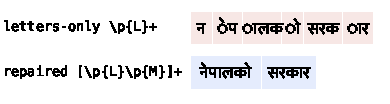
\includegraphics[width=0.95\columnwidth]{fig_split.pdf}
\caption{Pre-tokens of \emph{nep\=alko sark\=ar} (``government of Nepal'') under the letters-only regex of Llama-3 and Qwen and under the repaired regex. Dotted circles mark pre-tokens that begin with a dependent vowel sign.}
\label{fig:split}
\end{figure}

\paragraph{The floor, measured.} Table~\ref{tab:floor} gives the pre-token floor of Llama-3 and Qwen3 under their own letters-only regexes and under the repaired regex of each model. For both families the letters-only floor is about $2.2\times$, nearly three times the repaired floor ($2.77\times$ for Llama-3, $2.73\times$ for Qwen3), and above the premium of \texttt{o200k} ($1.61\times$).

\begin{table}[t]
\centering
\small
\begin{tabular}{lrrr}
\toprule
& Llama-3 & Qwen3 & \texttt{o200k} \\
\midrule
Current premium & 2.58 & 4.42 & 1.61 \\
Floor, letters-only regex & 2.19 & 2.17 & -- \\
Floor, repaired regex & 0.79 & 0.80 & 0.80 \\
\bottomrule
\end{tabular}
\caption{Nepali/English token premium on FLORES-200 devtest, and the pre-token floor under each regex (pre-tokens of Nepali / tokens of English): a lower bound on the premium of any vocabulary extension under that regex. Each model's floors use its own pattern (Qwen splits digits singly, Llama-3 in groups of up to three). Llama-3 and Qwen3 ship the letters-only regex; for \texttt{o200k}, which ships a mark-aware regex, the floor is under its own pattern.}
\label{tab:floor}
\end{table}

\paragraph{Released extensions sit on the floor.} Figure~\ref{fig:released} and Table~\ref{tab:released} (Appendix~\ref{app:released}) measure 12 released vocabulary extensions of letters-only models (15 extension--language pairs): eleven by \citet{yamaguchi2026lowres} on Llama-3, Llama-3.1, Qwen2.5 and Qwen3, ten of them for six scripts written with combining marks and one for Amharic, and the 61k-token in-place expansion of LFM2~\citep{smith2026inplace}, on four of its languages. Every Yamaguchi extension for a script with combining marks uses $1.013\times$ to $1.036\times$ as many tokens as its floor, closing 98.2--99.5\% of the gap between the base tokenizer and the floor. LFM2.5 sits at $1.07\times$ its floor for Hindi and $1.16\times$ for Nepali. Under the repaired regex the same text has 2.2 to 5.9 times fewer pre-tokens, so these extensions would have had that much more room. Yamaguchi's Amharic extension, for a script without combining marks, stays at $1.57\times$ its floor, and the repair does not move that floor. Two published releases fall below the letters-only floor: TituLLM~\citep{nahin-etal-2025-titullms} changed the regex (\S\ref{sec:related}), and SinLlama~\citep{aravinda2025sinllama} registered 11{,}080 strings as added tokens.

\begin{figure}[t]
\centering
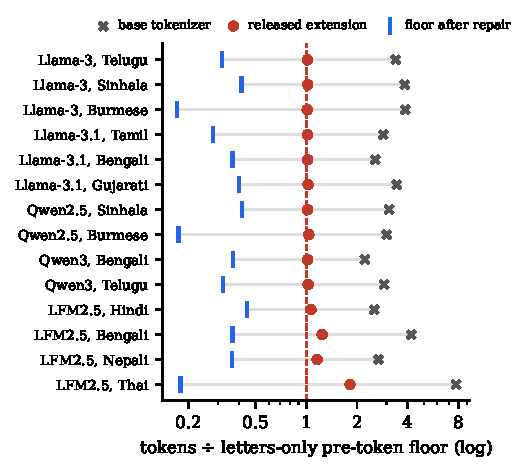
\includegraphics[width=0.95\columnwidth]{fig_released.pdf}
\caption{Released vocabulary extensions of letters-only models, on FLORES-200 devtest of each target language, relative to the letters-only pre-token floor. Ten extensions by \citet{yamaguchi2026lowres} (top) and LFM2.5~\citep{smith2026inplace} (bottom) move from the base tokenizer ($\times$) to the floor (\textcolor{red}{$\bullet$}) and stop there. The repaired regex would lower the floor to the blue tick. Full numbers, including the Amharic control, in Table~\ref{tab:released}.}
\label{fig:released}
\end{figure}
\section{Production audit}
\label{sec:audit}

We measured 33 released tokenizers on parallel FLORES-200 devtest text. Nine have identical token counts to another tokenizer on all 36 FLORES languages we measured (for example, Phi-4, OLMo-2 and Granite-4.1 all match \texttt{cl100k}; Qwen3 matches Qwen2.5; SmolLM3 matches Llama-3). We treat them as aliases, leaving 24 distinct tokenizers (Figure~\ref{fig:audit}; full table in Appendix~\ref{app:audit}). Two further tokenizers are not in the audit: Kimi-K3 requires executing remote code to load, which we did not run, and Mistral-Large-3 loaded through HuggingFace as a degenerate tokenizer, so we excluded it. We classify each tokenizer by its own pre-tokenizer configuration, not by family. Four SentencePiece and WordPiece tokenizers (XLM-R, mT5, NLLB-200, IndicBERTv2) do not reproduce their input on decoding, so their low premiums are not comparable compression results; Figure~\ref{fig:audit} marks them, and we exclude them from the analysis below.

\paragraph{The pre-token floor.} Let $P$ be a tokenizer's pre-tokenizer and $T$ the tokenizer. Summed over the 1{,}012 devtest sentences, we call $|P(\text{ne})|/|T(\text{en})|$ the \emph{pre-token floor} of $T$. The Nepali/English premium cannot go below it under any vocabulary extension that keeps the pre-tokenizer and leaves English tokenization unchanged (\S\ref{sec:ceiling}). It is a lower bound, not a value that extension is guaranteed to reach.

\begin{figure}[t]
\centering
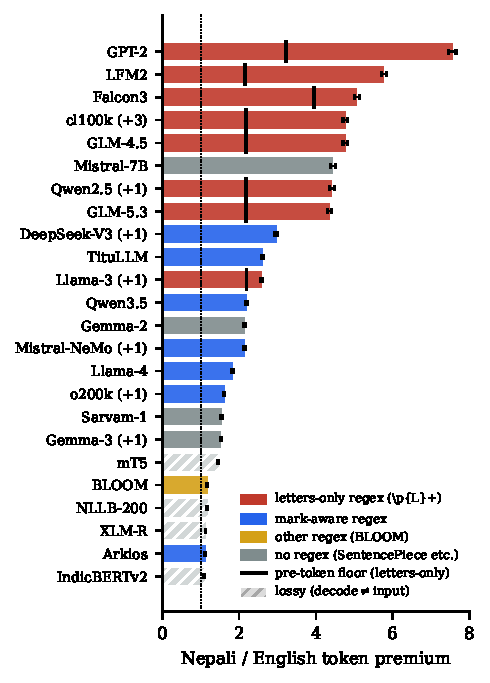
\includegraphics[width=\columnwidth]{fig_audit.pdf}
\caption{Nepali/English token premium of 24 distinct tokenizers (33 released tokenizers; ``+$n$'' counts aliases) on FLORES-200 devtest, with 95\% paired-bootstrap intervals. Black ticks mark the pre-token floor of each letters-only tokenizer: no vocabulary extension can move its bar to the left of the tick.}
\label{fig:audit}
\end{figure}

\paragraph{Every letters-only tokenizer has a floor of at least $2.15\times$.} Eight distinct tokenizers, covering 13 released names including GLM-5.3 and LFM2, use the letters-only class. Their premiums range from $2.58\times$ (Llama-3) to $7.55\times$ (GPT-2), and their pre-token floors from $2.15\times$ to $3.23\times$. Excluding GPT-2, a 2019 model that we include as a historical reference, the premiums of current letters-only models range from $2.58\times$ to $5.77\times$ (LFM2). The seven lossless tokenizers with a mark-aware regex range from $1.12\times$ (Arkios;~\citealp{regmi2026arkios}) to $2.97\times$ (DeepSeek-V3).

\paragraph{Decomposition.} Write the premium as
\begin{equation*}
\frac{|T(\text{ne})|}{|T(\text{en})|} = \underbrace{\frac{|P_{\text{rep}}(\text{ne})|}{|T(\text{en})|}}_{\text{base}} \cdot \underbrace{\frac{|P(\text{ne})|}{|P_{\text{rep}}(\text{ne})|}}_{\text{regex factor}} \cdot \underbrace{\frac{|T(\text{ne})|}{|P(\text{ne})|}}_{\text{vocabulary factor}},
\end{equation*}
where $P$ is the tokenizer's own pre-tokenizer and $P_{\text{rep}}$ is the repaired Llama-3 pattern (\S\ref{sec:method}), applied to every tokenizer. The numerator of the base term is therefore the same for all tokenizers; only the English token count varies. The base lies between $0.77$ and $0.80$ for every tokenizer, because English token counts barely differ. The regex factor is $0.98$--$1.02$ for mark-aware tokenizers, $2.77$--$2.79$ for the Llama-3/Qwen/\texttt{cl100k} pattern, and $4.06$ for the GPT-2 and Falcon3 patterns, which put every run of marks in a pre-token of its own. The vocabulary factor, tokens per pre-token, is what vocabulary extension can lower, and only down to 1.

Table~\ref{tab:decomp} shows where each tokenizer's premium comes from. For Llama-3 the vocabulary factor is $1.18$, the lowest in the audit: its 128k vocabulary already nearly covers Nepali pre-tokens, and almost all of its remaining premium is the regex factor. For Qwen and \texttt{cl100k} both factors matter. Among mark-aware tokenizers, the vocabulary factor varies from $1.43$ (Arkios, trained for Nepali) to $3.79$ (DeepSeek-V3): fixing the regex is necessary but does not by itself make a tokenizer good at Nepali.

\begin{table}[t]
\centering
\small
\setlength{\tabcolsep}{4pt}
\begin{tabular}{lrrrr}
\toprule
Tokenizer & Premium & Base & Regex & Vocab. \\
\midrule
GPT-2 & 7.55 & 0.80 & 4.06 & 2.34 \\
LFM2 & 5.77 & 0.78 & 2.77 & 2.68 \\
\texttt{cl100k} (+3) & 4.76 & 0.79 & 2.77 & 2.17 \\
Qwen2.5/3 & 4.42 & 0.78 & 2.79 & 2.03 \\
GLM-5.3 & 4.35 & 0.79 & 2.77 & 1.98 \\
Llama-3 & 2.58 & 0.79 & 2.77 & \textbf{1.18} \\
\midrule
DeepSeek-V3/V4 & 2.97 & 0.80 & 0.98 & 3.79 \\
Qwen3.5 & 2.20 & 0.78 & 1.02 & 2.76 \\
Llama-4 & 1.83 & 0.80 & 1.00 & 2.30 \\
\texttt{o200k} (+1) & 1.61 & 0.80 & 1.00 & 2.01 \\
Arkios & 1.12 & 0.79 & 0.99 & 1.43 \\
\bottomrule
\end{tabular}
\caption{Premium = base $\times$ regex factor $\times$ vocabulary factor, on FLORES-200 devtest, for 11 of the 15 letters-only and mark-aware tokenizers in the audit (top: letters-only; bottom: mark-aware). Arkios is from \citet{regmi2026arkios}. Vocabulary extension can only lower the last column, and not below 1.}
\label{tab:decomp}
\end{table}

\paragraph{Within-family changes.} Two families changed the regex between releases, together with the vocabulary. From Qwen3 to Qwen3.5 the Nepali premium halves, from $4.42\times$ to $2.20\times$; Qwen3.5's word branch is our repaired class with only the leading-character class left unchanged. \citet{land2026smallbugs} reported this change for Hindi. From Llama-3 to Llama-4 (which adopts \texttt{o200k}'s pattern) the premium falls from $2.58\times$ to $1.83\times$. In both cases the vocabulary also grew, so these are corroborating observations, not controlled comparisons; \S\ref{sec:compression} provides the controlled one.

\paragraph{Broken syllables.} Many Nepali tokens begin with a combining mark, which no well-formed Devanagari syllable does: 55\% of Llama-3's Nepali tokens, 32\% of Qwen3's and 30\% of \texttt{cl100k}'s (Appendix~\ref{app:audit}). The rate does not track the regex class. Mark-aware tokenizers show similar rates (26\% for \texttt{o200k}, 55\% for TituLLM, which keeps Llama-3's merges), because BPE also splits within words. \S\ref{sec:compression} shows how the rate moves under each retrofit.

\section{Repairing a deployed tokenizer}
\label{sec:method}

The repair has three parts: a one-class edit to the regex, new merges learned on top of the existing merge list, and an embedding initialisation that leaves the model's computation on old tokens unchanged.

\paragraph{Regex edit.} We admit \pM{} wherever the regex has a letter word class, and exclude it from the classes that would otherwise absorb a mark as a prefix or as punctuation. For the Llama-3/Qwen pattern this is two substitutions:
\begin{center}\small
\texttt{[\textasciicircum\textbackslash r\textbackslash n\textbackslash p\{L\}\textbackslash p\{N\}]?\textbackslash p\{L\}+}\\
$\downarrow$\\
\texttt{[\textasciicircum\textbackslash r\textbackslash n\textbackslash p\{L\}\textbackslash p\{M\}\textbackslash p\{N\}]?[\textbackslash p\{L\}\textbackslash p\{M\}]+}
\end{center}
and the same change in the punctuation branch \texttt{\textvisiblespace?[\textasciicircum\textbackslash s\textbackslash p\{L\}\textbackslash p\{N\}]+}. The optional leading class and the punctuation class must exclude \pM{}, so that a mark can only be matched by the word class and stays in one pre-token with the letters around it. Nothing else in the pattern changes, so digits, contractions, whitespace and punctuation are handled as before. We call the result the \emph{repaired regex}. Qwen3.5 independently shipped almost the same word branch (\S\ref{sec:audit};~\citealp{land2026smallbugs}).

\paragraph{Continued BPE, restricted to Devanagari.} Following \citet{purason-etal-2026-teaching}, we learn $K$ new merges on top of the existing ones. We pre-tokenize Nepali text with the arm's regex and segment every pre-token with the \emph{original} merges, which is how the deployed model sees it. Standard BPE over these segmentations, treating each base token as an indivisible symbol, then yields new merges, which we append after the existing ones. We discard any merge whose output contains no code point in U+0900--U+097F, together with merges that depend on it. At inference, BPE applies the lowest-ranked applicable merge first, so the original merges act before the new ones. The extended tokenizer reproduces the training procedure except in two cases: a new merge whose output string is already in the original vocabulary can let an original merge fire again afterwards, and under HuggingFace's \texttt{ignore\_merges} option (set for Llama-3) a pre-token that is itself a vocabulary entry is emitted directly. Neither case affects Proposition~\ref{prop:lossless}. We run the merge learning inside the HuggingFace Rust trainer by mapping each base token to a private-use code point. Learning $K{=}32{,}000$ merges on 1\,GB of Nepali text takes 1.7 to 3.4 minutes per tokenizer.

\RI{} and \RII{} use this identical procedure on identical text with identical $K$. The only difference is the regex used to pre-tokenize, both when learning merges and at inference.

\begin{proposition}[English invariance]
\label{prop:lossless}
Let $s$ be a string, after the tokenizer's normalizer, containing no code point of category \pM{} and no code point in U+0900--U+097F. Then the repaired tokenizer \RII{} and the original tokenizer produce identical token ids for $s$.
\end{proposition}
\begin{proof}
\emph{Pre-tokens.} The repaired regex differs from the original only in the three classes edited above, and each edited class differs from its original only on \pM{} characters. A regex match on $s$ consults only characters of $s$, and the order of the alternatives is unchanged. Since $s$ has no \pM{} character, both regexes produce the same pre-tokens.
\emph{Merges and vocabulary.} \RII{} differs from the original tokenizer only by appended merges and by the vocabulary entries they create, each of which contains a complete code point in U+0900--U+097F. A merge $(a,b)$ applies only where $a$ and $b$ are adjacent symbols of a pre-token, so its output is a contiguous substring of that pre-token's bytes. A vocabulary entry is emitted directly under \texttt{ignore\_merges} only if it equals the whole pre-token. Neither can happen for a pre-token of $s$, because UTF-8 is self-synchronising and $s$ contains no such code point. Each pre-token of $s$ is therefore encoded with original merges and original vocabulary entries only, exactly as by the original tokenizer.
\emph{Ids.} New ids are appended above the original ids, so all ids coincide.
\end{proof}

The proposition covers ASCII English and code, and every other script whose normalised text has no combining marks, including most Cyrillic, Han, Hangul and Ethiopic text. It does not cover Devanagari, even without marks: mark-free Devanagari words and Devanagari digits contain code points in U+0900--U+097F and change by design, since new merges apply to them. It also does not cover text with marks, such as Hindi or Latin written in decomposed form (NFD, e.g.\ \emph{caf\'e} with a combining acute). The Llama-3 tokenizer has no normalizer, so NFD input to a deployed Llama-3 \RII{} model falls outside the guarantee; Qwen3's tokenizer applies NFC itself, which composes most, but not all, combining marks. We normalise all our text to NFC. Empirically, \RI{} and \RII{} at $K{=}32{,}000$ give token ids identical to the original tokenizer on all 1{,}012 FLORES devtest sentences in English, Russian and Amharic, for both models. One Russian sentence contains a combining acute (U+0301) and so lies outside the proposition; its ids are nonetheless identical.

\paragraph{Embedding initialisation.} Each new token's constituents are the base tokens obtained by applying the original merges to the token's byte-level string; we do not decode it to text, which would turn tokens ending in a partial UTF-8 sequence into U+FFFD. Its input and output embedding rows are set to the mean of the constituent rows~\citep{gee-etal-2022-fast}. Original rows are untouched. Qwen3's embedding matrix has unused padding rows after its vocabulary, and the first new tokens reuse them. On any input whose ids are all original, the resized model therefore produces the same hidden states, and the same logits for every original token, as the base model. We check this numerically before training on an English probe sentence: the original-vocabulary logits are identical up to float error (maximum absolute difference $<10^{-4}$). The softmax denominator gains the new tokens' logits, so output probabilities are not identical, and continued pretraining is still needed.

\paragraph{Arms.} \RO{} (no extension) keeps the original tokenizer. \RI{} (extend) appends $K$ merges learned under the original letters-only regex: the standard recipe~\citep{purason-etal-2026-teaching,yamaguchi2026lowres}. \RII{} (repair + extend) switches to the repaired regex and appends $K$ merges learned under it. All arms then continue pretraining on the same bytes (\S\ref{sec:setup}).

\section{Experimental setup}
\label{sec:setup}

This section follows the second pre-registration amendment (Appendix~\ref{app:prereg}), which reduced the registered design to fit our budget before any continued-pretraining result was observed.

\paragraph{Models.} Llama-3.2-1B (base) and Qwen3-0.6B-Base, two widely used open models whose tokenizers ship the letters-only regex (\S\ref{sec:audit}). Both tie input and output embeddings. Qwen3-0.6B-Base uses the same tokenizer as Qwen3-1.7B-Base, on which we built the Qwen tokenizers of \S\ref{sec:compression}. The base models, without continued pretraining, are evaluated as a reference.

\paragraph{Data.} Nepali text is FineWeb-2 \texttt{npi\_Deva}; English is FineWeb-Edu (\texttt{sample-10BT}). We normalise to NFC, drop documents under 200 characters, remove exact duplicates, and drop every document that shares a whitespace 10-gram with FLORES-200 dev or devtest in Nepali or English. This also covers the Belebele passages, which are FLORES passages~\citep{bandarkar-etal-2024-belebele}, but not its questions or answers. Documents are stored one JSON-encoded document per line, so internal newlines are kept within a document. Before training, a 30\,MB held-out slice of each language is carved from the cleaned stream and never trained on. Statistics are in Appendix~\ref{app:data}.

\paragraph{Tokenizers.} \RI{} and \RII{} append $K$ merges learned on the same 1\,GB of Nepali text, taken from the start of the training stream. We sweep $K \in \{1, 2, 4, 8, 16, 32, 64\}\times 10^3$ for compression (\S\ref{sec:compression}) and use $K{=}32{,}000$ for training, as fixed in the pre-registration.

\paragraph{Continued pretraining.} Each arm is trained for one epoch on the \emph{same documents}: 1\,GB of Nepali and 1\,GB of English text, interleaved by document in one fixed order and separated by the model's end-of-text token. Because \RII{} encodes the same bytes in fewer tokens, it takes fewer optimisation steps and less compute; we report each arm's training FLOPs. To give an equal-compute view as well, \RO{} and \RI{} also save a checkpoint at the step count where \RII{} ends; their cosine schedules have not annealed at that point. Optimisation is identical across arms: sequence length 2{,}048, global batch 256 sequences (0.52M tokens), AdamW ($\beta = (0.9, 0.95)$, weight decay 0.1), gradient clipping at 1.0, 1\% linear warm-up, then cosine decay to 10\% of peak, bf16 autocast with fp32 master weights, on 4$\times$H200. The peak learning rate is fixed at $10^{-4}$ for every run and is not tuned. We train one seed (seed 0) per arm. Initialisation is deterministic and there is no dropout, so a second seed would change only the order of training windows and bf16 non-determinism.

\paragraph{Evaluation.} Because the arms tokenize differently, every metric is normalised by UTF-8 bytes, never by tokens. Every scored sequence is prefixed by the model's beginning-of-sequence token where it has one (Llama) and by its end-of-text token otherwise (Qwen), identically for every arm of a model.
\begin{itemize}
  \setlength\itemsep{0pt}
  \item \textbf{Bits per byte (BPB)} on the held-out native Nepali and English slices (4\,MB each), and on FLORES-200 devtest. The primary metric is \emph{byte-matched} BPB: each held-out document is split at whitespace into pieces of about 2{,}000 bytes, and every piece is scored independently, so every arm conditions on the same bytes of context. Token windows would give \RII{} more bytes of context per scored token. As a secondary metric, whole documents are scored with a sliding window of 2{,}048 tokens and stride 1{,}024.
  \item \textbf{Belebele}~\citep{bandarkar-etal-2024-belebele} \texttt{npi\_Deva} and \texttt{eng\_Latn}, zero-shot, scoring each of the four answer strings by its log-likelihood per byte given passage and question. Letter-choice prompting puts a 1B model at chance in both languages~\citep{regmi2026arkios}.
  \item \textbf{Translation}: FLORES-200 devtest Nepali$\leftrightarrow$English, 5-shot from FLORES dev, greedy decoding capped at 512 new tokens, chrF++.
  \item \textbf{Generation speed}: UTF-8 bytes generated per second in greedy continuation of FLORES dev Nepali sentences.
\end{itemize}
The equal-compute checkpoints are scored on BPB only.

\paragraph{Analysis.} The primary comparison is \RII{} against \RI{} and against \RO{} on byte-matched held-out Nepali BPB, at equal data (final checkpoints). We use a paired bootstrap over held-out pieces ($B{=}10{,}000$) of the per-piece BPB difference, and report the mean difference with its 95\% interval. We call \RII{} better if the interval of (\RII{} $-$ other) lies entirely below 0, non-inferior if it lies entirely below $+0.01$ bits per byte, and otherwise report no detectable difference. The same test on English pieces is the English control (\RII{} against \RO{}). With one seed, we cannot separate arm effects from data-order variance.

\section{Results}
\label{sec:results}

This section reports the controlled experiments: compression of the extended tokenizers and continued pretraining.

\subsection{Compression of repaired tokenizers}
\label{sec:compression}

Figure~\ref{fig:ksweep} sweeps the number of new merges $K$ for both models. Under the letters-only regex (\RI{}), extension saturates almost at once: for Llama-3 the first 1{,}000 merges take the premium from $2.58\times$ to $2.32\times$, and the next 63{,}000 only to $2.20\times$, within $0.01$ of the pre-token floor ($2.19\times$). For Qwen3, \RI{} cuts the premium from $4.42\times$ to $2.19\times$ by $K{=}16$k and then stops at $2.18\times$ against a floor of $2.17\times$. That \RI{} comes this close to its floor, rather than merely staying above it, is consistent with the small number of distinct Nepali pre-tokens the letters-only regex produces: the 1\,GB merge-training text has about 124k distinct pre-tokens under it, against 1.54M under the repaired regex. Under the repaired regex (\RII{}), the same merge budget keeps paying: $1.11\times$ at $K{=}16$k, $1.01\times$ at $32$k and $0.95\times$ at $64$k for both models, below parity with English and below \texttt{o200k}. At the pre-registered $K{=}32{,}000$, \RII{} encodes Nepali in 46\% of \RI{}'s tokens for both models.

All 28 extended tokenizers are lossless on the first 300 FLORES Nepali and English sentences (all 1{,}012 at $K{=}32{,}000$) and give token ids identical to the original tokenizer on all 1{,}012 English devtest sentences, as Proposition~\ref{prop:lossless} (for \RII{}) and its argument in \S\ref{sec:ceiling} (for \RI{}) require. FLORES dev, which we used to check the choice of $K$, gives the same picture within $0.02$.

\begin{figure}[t]
\centering
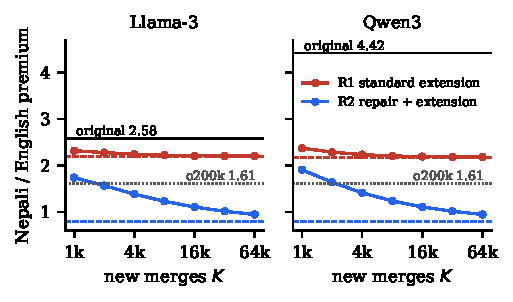
\includegraphics[width=\columnwidth]{fig_ksweep.pdf}
\caption{Nepali/English premium on FLORES-200 devtest after adding $K$ merges by continued BPE, under the letters-only regex (\RI{}) and the repaired regex (\RII{}). Dashed lines: pre-token floors of each regex, under each model's own pattern. Qwen3 tokenizers are built on Qwen3-1.7B-Base, whose tokenizer Qwen3-0.6B-Base shares. Shading: 95\% paired-bootstrap intervals.}
\label{fig:ksweep}
\end{figure}

\paragraph{Regex alone, and added tokens.} Two further arms separate the parts of \RII{}. Repairing the regex without adding merges (\RII{}, $K{=}0$) changes almost nothing: $2.61\times$ for Llama-3 (from $2.58\times$) and $4.42\times$ for Qwen3. Under the repaired regex, the old merges still tokenize Nepali words in old pieces; the regex only removes the ceiling that new merges would otherwise hit. Registering \RI{}'s new strings (31{,}999 of 32{,}000; one is a partial UTF-8 sequence) as added tokens instead of merges gives $2.35\times$ for Llama-3 and $2.19\times$ for Qwen3, no better than \RI{}. The gain of \RII{} therefore needs both the regex repair and new merges.

\paragraph{Broken syllables.} Extension under the letters-only regex makes syllable breaking worse. The share of Devanagari-bearing tokens (a slightly higher base than the all-token rate of \S\ref{sec:audit}) that begin with a combining mark rises from 57\% (Llama-3) and 33\% (Qwen3) to 67\% for both under \RI{}, because new merges can only build on mark-initial fragments. Under \RII{} it falls to 15\% and 12\%.

\paragraph{Other scripts.} We repeated the sweep for nine more languages, using the FineWeb-2 test split of each (25--361\,MB) to learn merges, with the same Devanagari-style output filter adapted to each script (Appendix~\ref{app:xling}). Table~\ref{tab:xling} (Appendix~\ref{app:xling}) gives the result at $K{=}32{,}000$; for example, \RII{} takes Tamil from $7.65\times$ to $1.02\times$ and Burmese from $11.62\times$ to $1.21\times$ on Llama-3, where \RI{} stops at $2.67\times$ and $3.02\times$. For every language written with combining marks except Thai, \RI{} stops at its floor and \RII{} reaches $0.88$--$1.24\times$. For the two scripts without combining marks, Amharic and Korean, \RI{} and \RII{} are identical at every $K$, as the mechanism predicts. All 108 extended tokenizers in this sweep are lossless and give English token ids identical to their base tokenizer on all 1{,}012 English devtest sentences.



\subsection{Continued pretraining}
\label{sec:cpt}

\begin{table*}[t]
\centering\small
\setlength{\tabcolsep}{4pt}
\begin{tabular}{lllrrrrrrrr}
\toprule
Model & Data & Arm & Tokens & ne BPB$\downarrow$ & en BPB$\downarrow$ & FLORES ne$\downarrow$ & Belebele ne & chrF ne$\to$en & chrF en$\to$ne & Gen.\ B/s \\
\midrule
Llama-3.2-1B & -- & base & 0 & 0.766 & 0.788 & 0.863 & 0.277 & 32.4 & 10.8 & 5327 \\
 & 1\,GB & \RO{} & 417M & \textbf{0.474} & 0.799 & 0.611 & 0.287 & 32.3 & 19.8 & 5147 \\
 & 1\,GB & \RI{} & 386M & 0.534 & 0.803 & 0.648 & 0.268 & 27.2 & 10.4 & 6354 \\
 & 1\,GB & \RII{} & 286M & 0.539 & 0.799 & 0.671 & 0.266 & 27.8 & 12.3 & 9398 \\
\addlinespace
 & 1\,GB + warm-up & \RO{} & 417M & 0.779 & 0.850 & 0.864 & 0.279 & 8.8 & 9.1 & 5349 \\
 & 1\,GB + warm-up & \RII{} & 286M & \textbf{0.527} & 0.840 & 0.652 & 0.283 & 16.2 & 15.4 & 11078 \\
\addlinespace
\midrule
Qwen3-0.6B & -- & base & 0 & 0.852 & 0.873 & 0.945 & 0.290 & 26.0 & 6.8 & 2186 \\
 & 1\,GB & \RO{} & 574M & \textbf{0.501} & 0.864 & 0.631 & 0.270 & 20.1 & 13.6 & 3089 \\
 & 1\,GB & \RI{} & 392M & 0.561 & 0.864 & 0.689 & 0.253 & 11.6 & 6.9 & 4972 \\
 & 1\,GB & \RII{} & 292M & 0.570 & 0.862 & 0.688 & 0.266 & 17.0 & 3.9 & 7454 \\
\addlinespace
\bottomrule
\end{tabular}
\caption{Continued pretraining on identical bytes per arm (one seed). BPB: bits per byte on held-out native text split into ${\sim}$2{,}000-byte pieces (primary metric) and on FLORES-200 devtest. Belebele: zero-shot accuracy (900 items, chance 0.25), scored on answer text. chrF++: 5-shot FLORES-200 devtest translation. Gen.\ B/s: UTF-8 bytes of Nepali generated per second (batch 64, greedy). Tokens: training tokens seen. Bold: best Nepali BPB within each block.}
\label{tab:cpt}
\end{table*}


Table~\ref{tab:cpt} reports every run. We state each comparison with the pre-registered paired bootstrap over held-out Nepali pieces (difference in bits per byte, 95\% interval).

\paragraph{Extension of either kind costs quality at this budget.} For both models, continued pretraining without new tokens (\RO{}) gives the lowest held-out Nepali BPB: 0.474 for Llama-3.2-1B (from 0.766) and 0.501 for Qwen3-0.6B (from 0.852). Both extended arms end higher, by similar amounts: \RI{} by $+0.060$ $[+0.059, +0.061]$ (Llama) and $+0.060$ $[+0.059, +0.061]$ (Qwen), \RII{} by $+0.066$ $[+0.065, +0.067]$ and $+0.070$ $[+0.068, +0.071]$ bits per byte. The cost therefore does not come mainly from the repair: it is almost as large ($+0.060$ against $+0.066$ and $+0.070$) when 32{,}000 tokens are added under the original regex. The new rows start from averages of existing rows; with 1\,GB of Nepali they do not catch up with the original vocabulary, which the base model already knows. \RO{} is also best at English-to-Nepali translation on both models.

\paragraph{Among extensions, the repair is close to standard extension and much cheaper.} \RII{} minus \RI{} on Nepali is $+0.0058$ $[+0.0049, +0.0067]$ bits per byte for Llama, inside the pre-registered non-inferiority margin of 0.01, and $+0.0094$ $[+0.0086, +0.0101]$ for Qwen, whose upper bound exceeds the margin by $0.0001$; under the pre-registered rule of amendment 2, \RII{} is non-inferior to \RI{} on Llama, and non-inferiority is not shown on Qwen, where the interval lies entirely above zero. On FLORES devtest the two are tied for Qwen (0.689 and 0.688). \RII{} reaches these numbers with 26\% (Llama) and 26\% (Qwen) fewer training tokens than \RI{}, is better on English for both models ($-0.003$ and $-0.002$, intervals excluding zero), and generates Nepali 1.48$\times$ (Llama) and 1.50$\times$ (Qwen) faster than \RI{}, and 1.83$\times$ and 2.41$\times$ faster than \RO{}, because each token carries more text. When \RI{} is stopped after the same number of steps as \RII{} and both are scored on the same 1\,MB of held-out Nepali, \RII{} is $+0.0056$ $[+0.0038, +0.0075]$ bits per byte worse for Llama and tied for Qwen ($+0.0000$ $[-0.0015, +0.0015]$); \RI{}'s learning rate has not annealed at that point.
%% EXPB-RESULTS

\paragraph{English is unaffected.} The registered English control holds: \RII{} minus \RO{} on held-out English is $+0.0003$ $[-0.0001, +0.0007]$ bits per byte for Llama (non-inferior) and $-0.0028$ $[-0.0031, -0.0025]$ for Qwen (better), as the invariance result predicts for the tokenizer and the equal English data in every arm predicts for the model.


\section{Discussion}
\label{sec:discussion}

\paragraph{Recommendations.} Before extending a letters-only model for a language with combining marks, compare the target text's pre-tokens with its tokens; if they are close, as for Llama-3 on Nepali, merges have little room. Under our recipes, plain continued pretraining gave the lowest held-out Nepali BPB, as \citet{zhao2024llamabeyond} found for Chinese, so extension needs another reason, such as token cost. Then the repair is worth considering: at matched steps it was within about 0.012 BPB of standard extension either way and needs 54\% fewer tokens for the same Nepali text, though we have not shown a latency gain for equally good outputs. We would use the Devanagari-only repair (untrained here; identical to ours on FLORES Nepali), load it with a class that does not rebuild its pre-tokenizer, and score models after the context they were trained with.

\paragraph{Why our sign differs from Regmi et al.} From scratch the wider class lowers Nepali BPB by 4.4\% at equal compute and still leads at equal bytes~\citep{regmi2026vowel}; retrofitted at equal bytes it is worse, and the gap decreases under longer training with repeated data \citep[cf.][]{shrestha2026papaya}: matched steps flip the sign on Qwen and halve the gap on Llama.

\section*{Limitations}

\begin{itemize}
  \setlength\itemsep{0pt}
  \item \textbf{The main hypothesis failed.} At our budget, neither extension recipe beat continued pretraining without new tokens on Nepali BPB. At equal bytes the repair was also worse than standard extension on both models; at matched steps it was better on Qwen and still worse on Llama.
  \item \textbf{Scale.} We adapt 1B- and 0.6B-parameter models with 1\,GB of text per language and one epoch; 1\,GB of Nepali also holds less content than 1\,GB of English~\citep{arnett-etal-2024-bit}. The registered 3\,GB runs were dropped for budget reasons, so we cannot say whether the gap between arms closes with more data; \citet{dagan2024getting} found recovery from a tokenizer change only after about 50B tokens in their code-adaptation setting.
  \item \textbf{Matched steps repeat data.} The matched-steps \RII{} runs reach \RI{}'s step count by seeing 35\% of their stream twice; they hold compute equal, not data, though repeating data for a few epochs costs little~\citep{muennighoff2023scaling}. We did not run \RO{} at matched steps, and Nepali is still a smaller share of \RII{}'s training tokens (26\% against 45\% for \RI{}).
  \item \textbf{Scoring two tokenizations.} For the seed-0 equal-bytes models we add the base tokenization to the canonical one, a partial step towards the marginal likelihood~\citep{cao-rimell-2021-evaluate,chirkova-etal-2023-marginalize}. It changes no score, because the models give the base tokenization almost no probability; this is a weak check, since nearer alternatives, such as splitting one new token, could still carry mass.
  \item \textbf{Few runs.} Every interval reflects only the sampling of evaluation text. In the Llama BOS rerun and on Qwen, every arm at $10^{-4}$ has two seeds, which differ by about $0.003$ or less per arm; the runs at $3{\times}10^{-4}$ have one.
  \item \textbf{Clustering.} Nepali intervals resample the 503 held-out documents; English intervals still cluster pieces by a length heuristic.
  \item \textbf{Learning rate.} We tried two learning rates, on Qwen only and with one seed at the higher one; continued-pretraining schedules matter~\citep{ibrahim2024simple}, and the English loss at the higher rate suggests forgetting. Moving from $10^{-4}$ to $3{\times}10^{-4}$ improved every arm by $0.02$ to $0.05$ without changing their order, so the best rate for each arm may differ from both and Llama was not tuned at all. Mean initialisation may also suit \RII{}'s long new tokens less well than \RI{}'s short ones~\citep{joshi2026beyondinit}.
  \item \textbf{BOS in training.} The main and warm-up Llama runs never saw BOS, which the registered evaluation puts first, so their registered scores and all their secondary metrics carry this artifact; the warm-up translation scores are unusable. The rerun with BOS in training resolves the main comparison, but only on BPB: we did not run Belebele, translation or generation for it, nor a warm-up version. Qwen has no BOS token and was not affected.
  \item \textbf{Weak secondary metrics.} Belebele accuracy is near chance for every model, translation scores come from a single greedy pass without intervals and keep only the first output line, which is empty whenever a model begins its answer with a newline (we did not count how often), and measured generation speed was taken on shared GPUs (Appendix~\ref{app:cptfull}).
  \item \textbf{Equal compute.} The equal-compute checkpoints of \RO{} and \RI{} are taken before their learning rate has fully decayed, and are scored on 1\,MB only.
  \item \textbf{Languages.} We train models for Nepali only. For other languages we report compression, and the general repair, which we trained and released, changes the tokenization of 61 FLORES-200 languages whose quality we did not measure, including Hindi and Thai, which Llama-3.2 officially supports. The cross-script tokenizers use a relaxed merge filter not covered by Proposition~\ref{prop:lossless} (Appendix~\ref{app:xling}).
  \item \textbf{Added tokens and segmentation.} We measured the added-token route around the floor only at the tokenizer level and trained no model with it; \citet{churchill2026reducing} add tokens post hoc to Llama 3.2 1B for whole characters, not words, and \citet{balde-etal-2024-adaptive} change how added tokens are matched. Our objection to it is segmentation, and we have no evidence that segmentation matters for quality. Whether the regex repair beats added tokens is untested.
  \item \textbf{Scoring context.} The BOS-consistent rerun scores every piece after BOS, but 1{,}756 of the 2{,}259 pieces start mid-document, a context these models never saw after BOS in training.
  \item \textbf{What would settle it.} A learning-rate sweep on both models, better embedding initialisation and a curve over data budgets would show whether \RO{}'s lead and the Llama gap persist.
\end{itemize}

\section*{Ethics and use of AI assistance}

All text and evaluation data are public (FineWeb-2, FineWeb-Edu, FLORES-200, Belebele) and used under their licences; we collected no data from people. Released Llama-derived tokenizers follow the Llama 3.2 Community License~\citep{llama32license}; Qwen3-derived tokenizers are Apache-2.0.

We used a large language model assistant extensively. Under our direction it wrote and ran the experiment code, searched the literature and drafted the text. We reviewed and approved the study design, the paper and all citations, and take responsibility for the content. The tokenizer-side numbers can be reproduced from public tokenizers and data with our released code, and every continued-pretraining statistic from the released per-piece scores.


\bibliography{refs}

\appendix
\section{Pre-registration history}
\label{app:prereg}

We pre-registered in three steps, in the public repository's git history, and report all three.

\begin{enumerate}
  \setlength\itemsep{0pt}
  \item Commit \texttt{bf5ebe4} (2026-10-04 17:59 NPT) registered hypotheses about the mechanism, a regex-only tokenizer ablation, a cross-script dose--response and from-scratch training. Our literature check then found that \citet{regmi2026vowel} had published the mechanism, the ablation, the cross-script analysis and a from-scratch downstream comparison five weeks earlier. We withdrew those hypotheses as contributions and do not report them as new.
  \item Commit \texttt{3c03367} (2026-10-04 18:16 NPT), before any model was trained or evaluated, registered the retrofit study reported here: arms \RO{}, \RI{}, \RII{} and the untrained base model as a reference; $K{=}32{,}000$ unless \RII{} saturated earlier on FLORES dev; equal-bytes continued pretraining; learning rate selected once per model on \RO{}; two seeds; primary metric held-out native Nepali BPB with a non-inferiority margin of 0.01 bits per byte; English BPB as a control; Belebele, translation and decoding speed as secondary. Its compression prediction (P1), including the letters-only floors, had already been measured when it was written, so we report P1 as a measurement, not a confirmed prediction.
  \item Commit \texttt{5ff74e8} (2026-10-04 19:50 NPT), amendment 2, was written after an internal review and before any continued-pretraining run had produced an evaluation. Earlier launches of continued pretraining were stopped by us before completion because of pipeline bugs, and none produced an evaluated checkpoint. The only evaluation run before the amendment, of the untouched base Llama-3.2-1B with a since-fixed document-prefix bug, is discarded. The amendment fixed the primary analysis as stated in \S\ref{sec:setup}.
\end{enumerate}

\paragraph{Deviations from the second registration (amendment 2).}
\begin{itemize}
  \setlength\itemsep{0pt}
  \item Qwen3-0.6B-Base replaces Qwen3-1.7B-Base (budget and time; same tokenizer).
  \item 1\,GB of Nepali and 1\,GB of English per arm replace 3\,GB and 3\,GB, with identical documents in every arm.
  \item A fixed learning rate of $10^{-4}$ for every run replaces selection on \RO{} from $\{3{\times}10^{-5}, 10^{-4}, 3{\times}10^{-4}\}$ by a 200-step pilot, which was never completed.
  \item One seed (seed 0) per arm replaces two.
  \item New: \RO{} and \RI{} are also checkpointed at \RII{}'s final step count (equal-compute view).
  \item New: byte-matched BPB on pieces of about 2{,}000 bytes is the primary metric; the registered sliding-window BPB becomes secondary.
  \item New: a paired bootstrap over held-out pieces, with explicit claim rules, is the primary test.
  \item The translation cap is 512 new tokens instead of 256, to avoid truncating Nepali output of \RO{}.
\end{itemize}

\paragraph{Pipeline bugs fixed before any reported run.} (1) Documents had been stored one per line with their internal newlines, so ``documents'' were paragraphs; they are now stored as one JSON-encoded document per line. (2) New-token embeddings had been initialised by decoding tokens to text, which turns partial UTF-8 tokens into U+FFFD; constituents now come from applying the original merges to the byte-level string. (3) The initialisation exactness check had covered Qwen's padding rows; it now covers only the original vocabulary. (4) Evaluation had prefixed documents with end-of-text, while base Llama expects its beginning-of-sequence token; we now use the latter where it exists, identically for every arm of a model.

Between the first two commits, the retrofit tokenizer code was tested on a 30\,MB sample of the FineWeb-2 Nepali \emph{test} split only.

\section{Data}
\label{app:data}

% filled after prep
\textcolor{red}{[data statistics pending]}


\section{Full audit}
\label{app:audit}

Table~\ref{tab:audit-full} lists every distinct tokenizer. Aliases are tokenizers whose token counts are identical to another tokenizer's on all 36 FLORES languages we measured; we did not compare token ids. Kimi-K3 (requires executing remote code) and Mistral-Large-3 (degenerate HuggingFace load) are not included.

\begin{table*}[t]
\centering\small
\setlength{\tabcolsep}{4pt}
\begin{tabular}{lllrrrrrl}
\toprule
Tokenizer & Aliases & Regex & $|V|$ & ne/en & 95\% CI & Floor & Mark-init. & Lossless \\
\midrule
IndicBERTv2 & -- & none & 250,000 & 1.09 & [1.08, 1.10] & -- & 6\% & no \\
Arkios & -- & mark-aware & 65,536 & 1.12 & [1.10, 1.13] & 0.79 & 15\% & yes \\
XLM-R & -- & none & 250,002 & 1.12 & [1.11, 1.14] & -- & 7\% & no \\
NLLB-200 & -- & none & 256,204 & 1.17 & [1.16, 1.18] & -- & 6\% & no \\
BLOOM & -- & other & 250,680 & 1.18 & [1.16, 1.19] & -- & 17\% & yes \\
mT5 & -- & none & 250,100 & 1.46 & [1.45, 1.47] & -- & 11\% & no \\
Gemma-3 & Gemma-4 & none & 262,145 & 1.53 & [1.51, 1.54] & -- & 9\% & yes \\
Sarvam-1 & -- & none & 68,096 & 1.54 & [1.52, 1.56] & -- & 14\% & yes \\
o200k & gpt-oss & mark-aware & 200,019 & 1.61 & [1.60, 1.63] & 0.80 & 26\% & yes \\
Llama-4 & -- & mark-aware & 201,135 & 1.83 & [1.81, 1.85] & 0.80 & 30\% & yes \\
Mistral-NeMo & Sarvam-M & mark-aware & 131,072 & 2.13 & [2.11, 2.15] & 0.79 & 33\% & yes \\
Gemma-2 & -- & none & 256,000 & 2.13 & [2.11, 2.15] & -- & 19\% & yes \\
Qwen3.5 & -- & mark-aware & 248,077 & 2.20 & [2.18, 2.23] & 0.80 & 19\% & yes \\
Llama-3 & SmolLM3 & letters & 128,256 & 2.58 & [2.55, 2.61] & 2.19 & 55\% & yes \\
TituLLM & -- & mark-aware & 170,497 & 2.60 & [2.57, 2.63] & 0.79 & 55\% & yes \\
DeepSeek-V3 & DeepSeek-V4 & mark-aware & 128,815 & 2.97 & [2.93, 3.00] & 0.80 & 38\% & yes \\
GLM-5.3 & -- & letters & 154,856 & 4.35 & [4.29, 4.40] & 2.19 & 33\% & yes \\
Qwen2.5 & Qwen3 & letters & 151,665 & 4.42 & [4.36, 4.47] & 2.17 & 32\% & yes \\
Mistral-7B & -- & none & 32,768 & 4.44 & [4.38, 4.50] & -- & 29\% & yes \\
GLM-4.5 & -- & letters & 151,365 & 4.76 & [4.71, 4.82] & 2.19 & 30\% & yes \\
cl100k & Phi-4, OLMo-2, Granite-4.1 & letters & 100,277 & 4.76 & [4.71, 4.82] & 2.19 & 30\% & yes \\
Falcon3 & -- & letters & 131,072 & 5.07 & [5.00, 5.14] & 3.96 & 28\% & yes \\
LFM2 & -- & letters & 64,400 & 5.77 & [5.70, 5.84] & 2.15 & 24\% & yes \\
GPT-2 & -- & letters & 50,257 & 7.55 & [7.46, 7.65] & 3.23 & 19\% & yes \\
\bottomrule
\end{tabular}
\caption{All 24 distinct tokenizers (33 released tokenizers) on FLORES-200 devtest. Aliases: tokenizers whose token ids are identical on every devtest sentence of five languages (Appendix~\ref{app:audit}). Regex: letters-only, mark-aware, other, or none (no regex pre-tokenizer). ne/en: Nepali/English token premium with 95\% paired-bootstrap interval. Floor: pre-token floor under the tokenizer's own regex, a lower bound on the premium of any merge-based extension (letters-only and mark-aware tokenizers only). Mark-init.: share of Nepali tokens whose first character is a combining mark. Lossless: decoding reproduces the input on 200 Nepali sentences. Arkios is from \citet{regmi2026arkios}. Hugging Face repositories are listed in the released code.}
\label{tab:audit-full}
\end{table*}


\section{Cross-script sweep}
\label{app:xling}

For each language we downloaded the FineWeb-2 \emph{test} split, normalised it to NFC, and removed documents that share a whitespace 10-gram with that language's FLORES-200 dev or devtest (for Thai, which has no spaces, we also checked 50-character overlaps and found none). The resulting merge-learning text ranges from 25\,MB (Amharic) to 361\,MB (Bengali), less than the 1\,GB used for Nepali; Sinhala and Amharic \RII{} may be limited by it. $K{=}4$k and $16$k are prefixes of one $32$k run.

The Nepali filter keeps a new merge only if its output contains a complete Devanagari character. For scripts that the base vocabularies cover poorly, many characters are themselves split into byte pieces, and this filter would drop the first byte-level merge of a character and every merge built on it (for Sinhala \RII{}, only 13{,}530 of 32{,}000 merges survived). For the cross-script sweep we therefore also keep merges whose output is a byte piece of a target-script character. Such merges can only fire on target-script bytes, so the English guarantee is unaffected; we verified English token ids on all 1{,}012 sentences for every tokenizer. Hindi uses the same script as Nepali, and its new merges also change Nepali tokenization; we did not measure that interaction.

\section{Released extensions}
\label{app:released}

\begin{table}[h]
\centering
\small
\setlength{\tabcolsep}{3pt}
\begin{tabular}{llrrr}
\toprule
Base & Lang. & Tokens/floor & Gap closed & Room \\
\midrule
Llama-3-8B & te & 1.016 & 99.3\% & 3.16$\times$ \\
Llama-3-8B & si & 1.021 & 99.3\% & 2.42$\times$ \\
Llama-3-8B & my & 1.013 & 99.5\% & 5.87$\times$ \\
Llama-3.1-8B & ta & 1.018 & 99.1\% & 3.58$\times$ \\
Llama-3.1-8B & bn & 1.020 & 98.7\% & 2.74$\times$ \\
Llama-3.1-8B & gu & 1.026 & 98.9\% & 2.52$\times$ \\
Qwen2.5-7B & si & 1.019 & 99.1\% & 2.40$\times$ \\
Qwen2.5-7B & my & 1.036 & 98.2\% & 5.72$\times$ \\
Qwen3-14B & bn & 1.019 & 98.5\% & 2.71$\times$ \\
Qwen3-14B & te & 1.027 & 98.6\% & 3.11$\times$ \\
\midrule
LFM2 (2.5) & hi & 1.068 & 95.5\% & 2.24$\times$ \\
LFM2 (2.5) & ne & 1.160 & 90.5\% & 2.77$\times$ \\
LFM2 (2.5) & bn & 1.243 & 92.4\% & 2.74$\times$ \\
LFM2 (2.5) & th & 1.819 & 87.9\% & 5.57$\times$ \\
\midrule
Llama-3.1-8B & am & 1.573 & 93.8\% & 1.00$\times$ \\
\bottomrule
\end{tabular}
\caption{Released vocabulary extensions that keep the letters-only regex, on FLORES-200 devtest of the target language. Tokens/floor: extended-tokenizer tokens divided by pre-tokens under its own regex (at least 1 by construction). Gap closed: share of the base-to-floor gap that the extension removed. Room: floor under the letters-only regex divided by floor under the repaired regex. Top block: \citet{yamaguchi2026lowres}; middle: LFM2.5~\citep{smith2026inplace}; bottom: Amharic, which has no combining marks (control).}
\label{tab:released}
\end{table}


\end{document}
